\documentclass[11pt]{report}
\usepackage[utf8]{inputenc}
\usepackage[T1]{fontenc}
\usepackage[unicode=true]{hyperref}
\usepackage{lmodern}
\usepackage[french]{babel}

%%% PAGE DIMENSIONS
\usepackage{geometry}
\geometry{a4paper}
\geometry{top=2.5cm, bottom=2.5cm, left=4.5cm , right=3.5cm}
\usepackage{graphicx}


%%% PACKAGES
\usepackage{booktabs} % for much better looking tables
\usepackage{array} % for better arrays (eg matrices) in maths
\usepackage{paralist} % very flexible & customisable lists (eg. enumerate/itemize, etc.)
\usepackage{verbatim} % adds environment for commenting out blocks of text & for better verbatim
\usepackage{subfig} % make it possible to include more than one captioned figure/table in a single float
\usepackage{amssymb,amsmath}
\usepackage{xcolor}
\usepackage{sistyle}
\usepackage{shorttoc}
\usepackage{titlesec}
\usepackage{titletoc}
\usepackage{listings}

\hypersetup{breaklinks=true,
            pdfauthor={Thibault Deutsch (deutsc\_t); Ilan Dubois (dubois\_o); Arthur Douillard (douill\_a); Axel Mendoza (mendoz\_a)},
            pdftitle={Rapport de projet},
            colorlinks=true,
            citecolor=blue,
            urlcolor=blue,
            linkcolor=black,
            pdfborder={0 0 0}}

\setlength{\parskip}{6pt plus 2pt minus 1pt}
\setlength{\emergencystretch}{3em}  % prevent overfull lines

\setcounter{secnumdepth}{3}
\setcounter{tocdepth}{4}
\renewcommand{\thechapter}{\Roman{chapter}}
\renewcommand{\thesection}{\arabic{section}.}
\renewcommand{\thesubsection}{\arabic{section}.\arabic{subsection}}
\renewcommand{\thesubsubsection}{\arabic{section}.\arabic{subsection}.\arabic{subsubsection}}

\usepackage{fancyhdr} % This should be set AFTER setting up the page geometry
\pagestyle{fancy}
\fancyhead[L]{(Neurone)\up{*}}
\fancyhead[C]{}
\fancyhead[R]{Oh! Ça seRt}

\title{Rapport de projet}
\author{Thibault Deutsch (deutsc\_t) \and Ilan Dubois (dubois\_o) \and Arthur Douillard (douill\_a) \and Axel Mendoza (mendoz\_a)}
\date{10 décembre 2014}

\dottedcontents{chapter}%
  [\dimexpr 10mm]
  {}
  {\dimexpr 10mm}
  {3.2mm}

\dottedcontents{figure}%
  [\dimexpr 15mm]
  {}
  {\dimexpr 15mm}
  {3.2mm}

\begin{document}
\renewcommand{\labelitemi}{$\bullet$}

\begin{titlepage}
\newcommand{\HRule}{\rule{\linewidth}{0.5mm}} % Defines a new command for the horizontal lines, change thickness here

%----------------------------------------------------------------------------------------
%	LOGO SECTION
%----------------------------------------------------------------------------------------
\flushright

\includegraphics[width = 4.5cm]{epita.png}\\[0.5cm] % Include a department/university logo - this will require the graphicx package

%----------------------------------------------------------------------------------------
%	HEADING SECTIONS
%----------------------------------------------------------------------------------------
\textsc{\Large Rapport de projet}\\[0.15cm] % Major heading such as course name
\textsc{\large 2\up{ème} année du cycle préparatoire}\\[3cm] % Minor heading such as course title

%----------------------------------------------------------------------------------------
%	TITLE SECTION
%----------------------------------------------------------------------------------------
\center
\HRule \\[0.5cm]

\includegraphics[width = 10cm]{logo.png}\\[1cm]
\textsc{\Large Un OCR développé en C}\\[0.1cm]
\large 10 décembre 2014\\[0.1cm]
\HRule \\[3cm]

\Large
\textbf{Thibault Deutsch} (\emph{deutsc\_t}) \\
\textbf{Ilan Dubois} (\emph{dubois\_o}) \\
\textbf{Arthur Douillard} (\emph{douill\_a}) \\
\textbf{Axel Mendoza} (\emph{mendoz\_a})\\[2cm]

%----------------------------------------------------------------------------------------
\vfill % Fill the rest of the page with whitespace

\end{titlepage}

\newpage
\pagenumbering{arabic}
\tableofcontents

\chapter{Introduction}

Ce document est le rapport de projet. Son objectif est de présenter une synthèse du travail fournit par l’équipe (Neurone)\up{*}.\ Ce groupe est composé de quatre étudiants en deuxième année du cycle préparatoire de l’EPITA : Thibault DEUTSCH (deutsc\_t), Ilan DUBOIS (dubois\_o),  Axel MENDOZA (mendoz\_a), et Arthur DOUILLARD (douill\_a).

Le projet consiste en la réalisation d’un logiciel de reconnaissance optique de caractères (OCR, en anglais \emph{optical character recognition}). Le but de ce logiciel est de convertir un document numérisé, à l'aide d'un scanner, en un fichier numérique modifiable. Pour cela, le programme doit être capable d'extraire la structure du document et de reconnaître les différents caractères.

Nous devons réalisés ce projet en C. Son développement se déroule sur une période d’environ trois mois, en équipe de quatre personnes. Ce projet à pour objectifs, outre l'apprentissage du C, de nous familiariser avec le développement sur environnement GNU/Linux, le respect d'un cahier des charges, ains que le travail de groupe sur un projet commun.

Nous avons choisi d’appeler notre groupe (Neurone)\up{*} en référence à l’étoile de Kleene vu en conférence de THLR\footnote{Théorie des langages rationnels}. Le choix du nom du projet a été fait dans un objectif comique, ``Oh ça sert'' a bien sûr pour initiales OCR\footnote{Ce n'est pas immédiat, mais tout de même...}.

Vous trouverez dans la suite de ce rapport une présentation détaillée sur les différentes dimensions du développement.

\newpage
\section{Présentation des membres du groupe}

\subsection{Thibault Deutsch}

Je suis passionné d’informatique depuis la cinquième. Cette passion m’a permis de développer très rapidement de nombreuses connaissances, notamment en m’impliquant dans des projets libres mais également par le biais de ma première et terminal S SI où j’ai été amené à diriger deux projets conséquents. De mes expériences antérieures, j’ai appris que chaque projet était un apport de connaissance très important, mais aussi qu’il doit être dirigé pour ne pas divaguer. C’est pourquoi je me suis proposé comme chef de projet pour mon projet de SUP.

Après le succès du projet TROMA, j'ai décidé de réitérer l'expérience. Je pense avoir encore énormément de chose à apporter à ce groupe, notamment ma maitrise du C. J'espère que l'équipe profitera de mes connaissances et de mes astuces pour progresser dans tous les domaines de la conception d'un projet.

\subsection{Ilan Dubois}

Je m’intéresse à l’informatique depuis le collège. En effet, pendant cette période j’avais entrepris de faire un site traitant des jeux-vidéo avec quelques amis. J’ai donc dû m’intéresser au Web et j’ai administré ce site pendant 4 ans. J’ai récemment arrêté car il devenait difficile de concilier les divers emplois du temps. En regardant différents tutoriels, je me suis progressivement intéressé aux systèmes Unix. Je m’intéresse aussi au monde du logiciel libre, et aux bénéfices que leur utilisation peut nous apporter.

Aujourd'hui, j'aimerais améliorer mes compétences en C/C++ pour pouvoir participer à des projets libres ou en lancer certains. C'est une des raisons qui fait que j'apprécie particulièrement ce projet. Je met aussi en place un certain de nombre de choses sur mon serveur dédié pour progresser dans la maîtrise de système UNIX, une Debian en l'occurence.

\subsection{Arthur Douillard}

Passionné d’informatique de 19 ans, venant d’une prépa et voulant pouvoir coder de façon sérieuse, je suis venu à l’EPITA pour pouvoir exercer ma passion : L’informatique et pouvoir concrétiser mon rêve : devenir roboticien. Je suis moins doué que mes camarades en programmation mais je compte bien combler ce déficit le plus vite possible. L’OCR a été donc un baptême du feu très intéressant, où j’ai pu découvrir nombres d’aspects du C que j’ignorais.

\subsection{Axel Mendoza}

Mon nom est Axel Mendoza, j'ai 20 ans et je n'ai jamais touché à l'informatique avant mon entrée à l'Epita. Malgré tout, depuis que j'ai découvert ce domaine, j'y porte un grand intérêt car l'Epita constitue un accédé à un  métier d'ingénieur qui est une profession d'avenir. 

L'année dernière, j'ai eu le malheur de faire partie d'un groupe de projet où mes partenaires n'ont pas eu le courage de suivre le rythme de travail que l'ont nous a imposé. Mais je n'ai pas perdu espoir pour autant, je suis parvenu à présenter un jeu plutôt convenable lors de ma soutenance finale. Cette année tout à changer ! Mes partenaires sont motivés, sympathique et ne refusent jamais de fournir un peu d'aide à quelqu'un qui ne parvient pas a trouver la solution à un problème. Pour finir, je dois reconnaître que le langage C me plaît plus que le C\# et que le fait de travailler sur un OCR va indéniablement élargir nos domaines de compétence.

\section{Répartition des tâches}

La répartition des tâches est présentée dans le tableau en figure~\ref{tab}.

\medskip

\colorlet{darkgreen}{green!60!black}

\begin{figure}[htbp]
\centering
\begin{tabular}{ | c || c | c | c | c | }
\hline Tâches & Thibault & Ilan & Arthur & Axel \\
\hline Pré-traitement & & & \textcolor{darkgreen}{X} & \textcolor{darkgreen}{X} \\
\hline Analyse et segmentation & \textcolor{darkgreen}{X} & \textcolor{darkgreen}{X} & & \\
\hline Reconnaissance des caractères & \textcolor{darkgreen}{X} & \textcolor{darkgreen}{X} & & \\
\hline Interface graphique & & & \textcolor{darkgreen}{X} & \textcolor{darkgreen}{X} \\
\hline Site web & & & \textcolor{darkgreen}{X} & \\
\hline
\end{tabular}
\caption{Répartition des tâches sur l'ensemble de la durée du projet}
\label{tab}
\end{figure}

\chapter{Pré-traitement}

Les filtres et masques flou, dans un logiciel à reconnaissance de caractère, sont utilisés lors du pré-traitement. Cette étape préalable à détection des caractères est indispensable. En effet, son but est d’adaptés les caractéristiques de l'image à notre algorithme qui segmentera l'image en lignes et en caractères. L'image subit alors plusieurs transformations. En premier lieu, nous devons saturé les couleurs de celle-ci afin d'obtenir uniquement du noir et du blanc. Le second traitement consiste à éliminer le bruit, grâce à l'application d'un filtre sur notre image d'origine. 

Vous trouverez dans la suite de ce chapitre des explications détaillées sur l'ensemble des techniques mises en oeuvre.

\section{Binarisation}

La première étape de la binarisation est de passer l’image en niveaux de gris. Nous avons choisi de faire une moyenne pour obtenir l’image en niveaux de gris, cela nous semblait suffisant. Ensuite la partie intéressante de la binarisation arrive : transformer cette image qui est en niveaux de gris en une image binaire.

\subsection{Seuil fixe}

Notre première idée fut d'utiliser un seuil fixe. Il s'agit de la méthode la plus classique. Les 128 niveaux de gris les plus clairs deviennent blancs, et les 128 niveaux de gris les plus foncés deviennent noir. Cela revient à prendre un seuil de 127. Cette méthode fonctionne sur des images à fort contraste (texte sombre et fond clair par exemple). Cependant si l'on prend, par exemple, une image avec un fond et un texte de couleurs sombre (mais qui reste lisible par l’être humain), cette méthode de binarisation génère une image soit toute blanche, soit toute noire.

\begin{figure}[htbp]
\centering
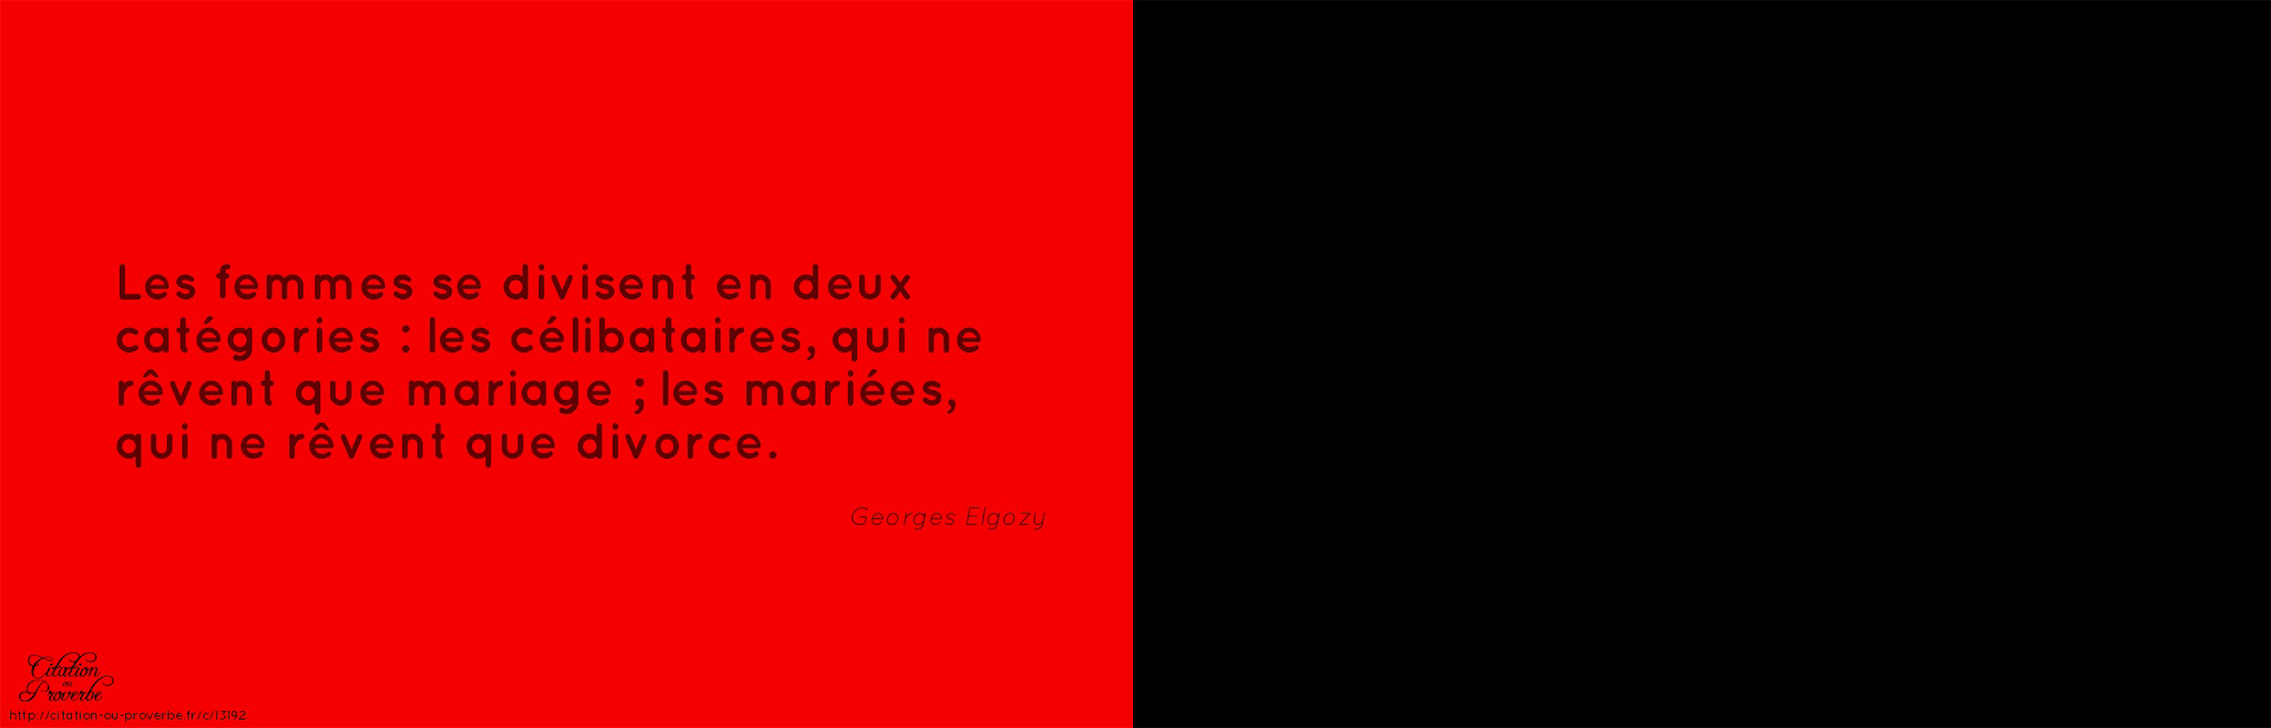
\includegraphics[width=10cm]{b_fixed.png}
\caption{Binarisation à seuil fixe}
\end{figure}

Nous avons donc décider d'abandonner cette méthode afin de nous tourner vers un algorithme capable d'adapter le seuil en fonction de l'image.

\subsection{Méthode d'Otsu}

L'algorithme que nous avons décider d'utiliser s'appelle la méthode d'Otsu, du nom de son initiateur japonais Nobuyuki Otsu. Cette algorithme considère que l’image que l’on souhaite binariser n’est composée que de deux types de pixels, le premier-plan et l’arrière-plan. Ce qui est exactement ce que l’on veut sachant que l’on travaille sur des images constitués de textes (premier-plan) et d’un fond (arrière-plan). En partant de ce principe, la méthode d'Otsu calcule le seuil optimal qui sépare ces deux plans.

Nous réalisons l'histogramme des couleurs de notre image en niveaux de gris. Ainsi pour on obtient pour chaque niveau de gris la quantité de fois qu'il apparaît dans l'image. Ce résultat est utilisé pour calculer sa probabilité d’apparaître dans l’image. C'est ensuite cette probabilité qu’on utilisera dans le calcul de la variance nécessaire à la formule d’Otsu :

\[ \sigma ^{2}_{w} \left( t\right) = w_{1}\left( t\right) \sigma ^{2}_{1}\left( t\right) + w_{2}\left( t\right) \sigma ^{2}_{2}\left( t\right) \]

\begin{description}
\item[$w_{i}$] représentent la probabilité d'être dans l'arrière-plan ou le premier-plan.
\item[$\sigma ^{2}_{i}$] représentent les variances de ces deux catégories.
\end{description}

\medskip

Ensuite nous procédons à une binarisation de la même manière que celle mentionnée précédemment mais en utilisant le seuil calculer par l'algorithme d'Otsu. Ainsi nous sommes sûr que la binarisation est adapté à l’image fournie par l'utilisateur.

\begin{figure}[htbp]
\centering
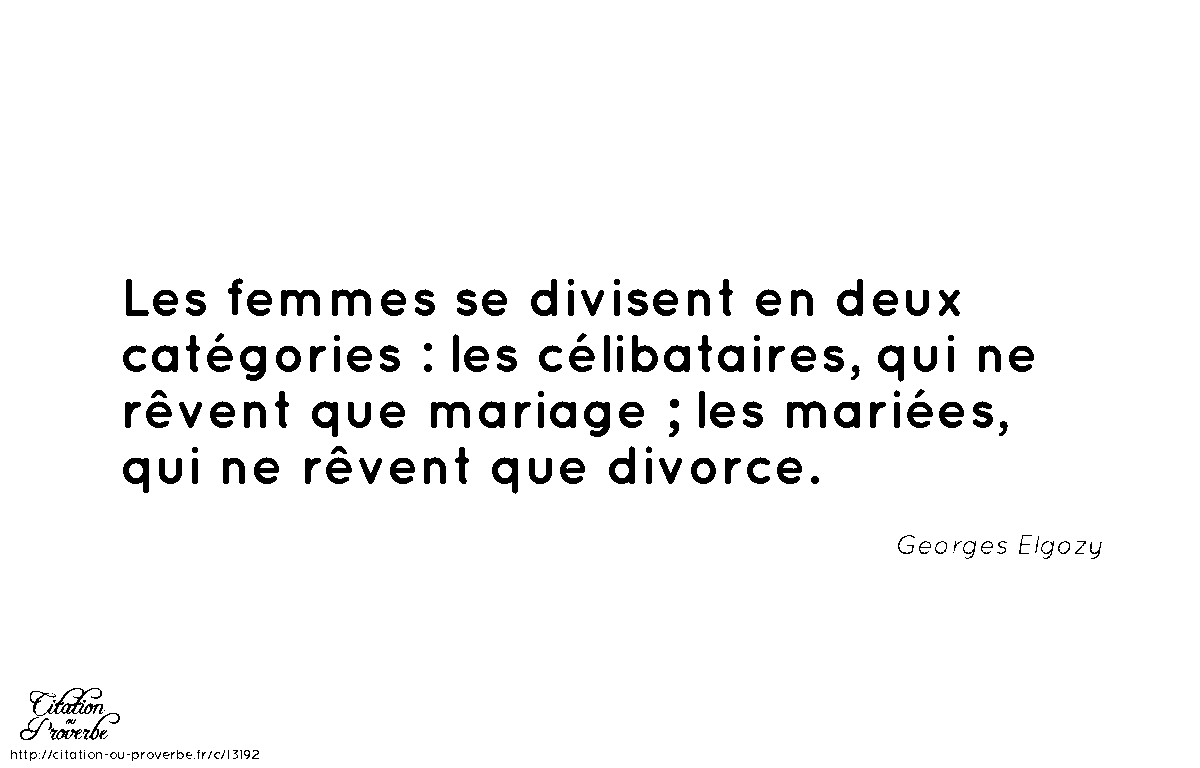
\includegraphics[width=10cm]{b_otsu.png}
\caption{Binarisation utilisant la méthode d'Otsu}
\end{figure}

\section{Filtres}

Après m'être documenté sur l'élimination du bruit, à l'aide de documents se réfèrent au bruit dans les images, aux différents problèmes récurrents en imagerie numérique et aux méthode utilisés pour résoudre ces problèmes. J'ai choisit deux méthodes pour éliminer le bruit, le filtre moyen qui est un filtre basique à but purement pédagogique, et le filtre gaussien qui effectue un flou plus sophistiqué et mieux adaptés à notre projet. 

L'image à traiter proviendra d'un scanner, nous remarquerons que cette image aura certains défauts qu'il faudra éliminer à l'aide du flou en question. En effet, si l'image est floue, le passage d'une valeur à l'autre se fait plus progressivement et l'algorithme de détection de caractères et donc plus optimale. Mathématiquement, une image est rendue floue en utilisant un filtre qui élimine les détails associés à de plus hautes fréquences qui constitue le bruit et les parasites en imagerie numérique qui polluent l'information. Malheureusement, nous ne pouvons appliquer directement un filtre passe-bas ``classique'' sur notre image car cette méthode risque de supprimer les petits caractères isolés tel que les points sur les ``i'' ou les accents. C'est pour cela que nous avons choisit d'appliquer une méthode qui adapte le flou en fonction de la nature des pixels voisins.

\subsection{Matrice de convolution et flou gaussien}

Nous allons aborder maintenant le principe du flou gaussien. En premier lieu, il nous faut définir l'opération mathématique appelée ``convolution'' utilisé dans tout les filtres dit linéaires. Lorsqu'il s'agit de données numérisés comme dans notre cas en traitement d'image, la relation entre les valeurs des pixels d'entrée et celle des pixels de sortie est décrite par un tableau de nombres, généralement carré, appelé matrice de convolution.  Le filtre gaussien, comme son nom l'indique, utilise la loi de probabilité de Gauss et la courbe gaussienne. Le principale problème de ce filtre est que l'application directe de la formule gaussienne nécessite un temps de calcul considérable. Heureusement, certains algorithmes effectuent ce calcul à l'aide d'approximations de plus en plus précises qui améliore grandement la complexité de l'algorithme qui applique ce filtre sur notre image.

\begin{figure}[htbp]
\centering
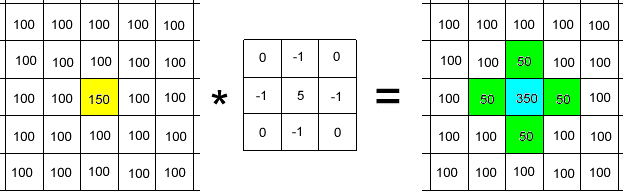
\includegraphics[width=10cm]{matconvol.jpg}
\caption{Application d'une matrice de convolution}
\end{figure}

Au départ nous avons utilisé un filtre moyen, qui calcule les composants de chaque pixels en fonctions de ses pixels directement adjacents mais nous n'étions pas convaincue en ce qui concerne  l'efficacité de ce flou. La première méthode du filtre gaussien, consiste à appliquer une matrice de convolution de dimension impaire ($3 \times 3, 5 \times 5, …$). Une matrice de convolution de dimension $3 \times 3$ nous a parut plus performant. En effet, plus la dimension de la matrice est élevée, plus la perte d'information est importante. Chaque pixels de l'image est modifié en fonction des composantes des pixels environnants. Plus la matrice de convolution est grande, plus les composantes des  pixels seront influencées par les pixels environnants. En somme, plus notre matrice de convolution est grande, plus le flou est important. En appliquant la matrice sur un pixel, les produits des composantes des pixels voisins avec la valeur de la matrice correspondante. Le résultat est en suite divisé par la somme des valeurs de notre matrice de convolution. 

\begin{figure}[htbp]
\centering
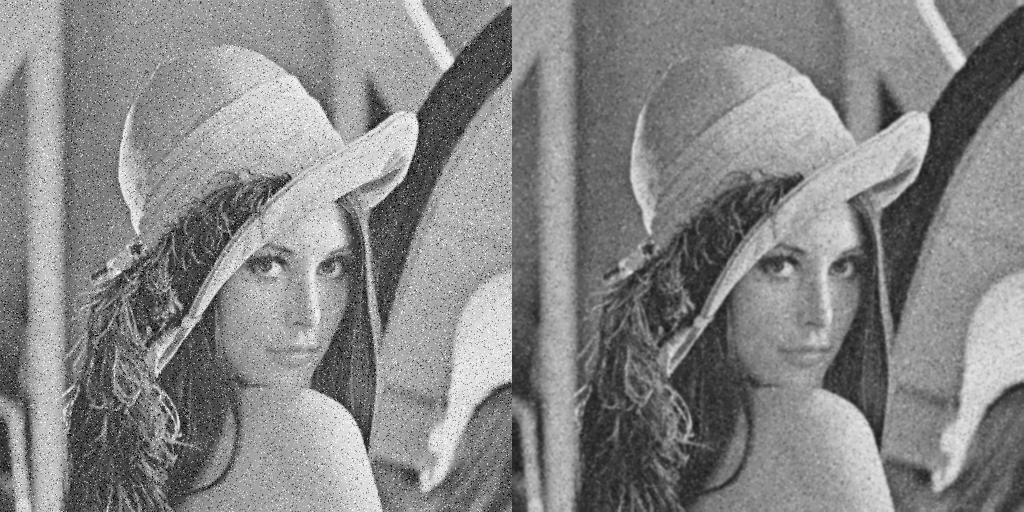
\includegraphics[width=10cm]{filtre_gaussien.png}
\caption{Application du filtre gaussien sur une image bruitée}
\end{figure}

Le principe du filtre gaussien est donc le suivant : on parcours l'image pixel par pixel, en appliquant le masque sur chaque pixels et ses voisins. On stocke le résultat des calculs effectuer sur les pixel dans une variable constituant un tableau à deux dimensions et on retourne cette variable. Nous avons également utilisé une fonction qui nous renvoi le symétrique d'un pixel par rapport à la matrice de convolution lorsque ce pixel était en dehors de notre image. Lorsque l'on veut appliquer le masque sur un pixel au bord de l'image, on tente de sommer les composantes d'un pixel qui n'existe pas. Mais lorsque l'on somme le pixel symétrique à celui-ci et qu'on le divise par le coefficient au même emplacement dans le masque, le résultat n'est pas erroné.
\subsection{Filtre médian}

Lors de l'implémentation de la segmentation de l'image, nous avons remarqué que lorsque l'image contient des grains de bruits à plusieurs pixels adjacents, l'application d'un filtre gaussien $5 \times 5$ n'élimine pas correctement les informations parasites. De plus, le filtre gaussien rend l'image flou. Lorsque l'on parcours l'histogramme de notre image pour détecter les contours des paragraphes, lignes ou caractères, notre algorithme de détection considérait alors ces grains de bruits comme de minuscule caractères.

Nous avons donc décider d'ajouter un filtre médian à notre logiciel. Cette méthode consiste à appliquer une matrice de convolution impaire sur chaque pixel de l'image comme précédemment avec le filtre gaussien. Nous avons put remarquer qu'un masque $3 \times 3$ appliqué à notre image suffisait pour faire disparaître les amas important de pixel crée par le bruit. 

Lorsque l'on traite un pixel, nous allons ajouter dans une liste les pixels environnant celui-ci. Nous devons alors utiliser un tri à bulle qui est amplement suffisant pour une petite collection de données, afin de trouver le pixel médian de notre liste. Il faut impérativement allouer un tableau tampon où l'on stocke la nouvelle valeur de notre pixel. Pour finir, on libère l'image courante puis la remplace par notre tableau alloué précédemment.

\begin{figure}[htbp]
\centering
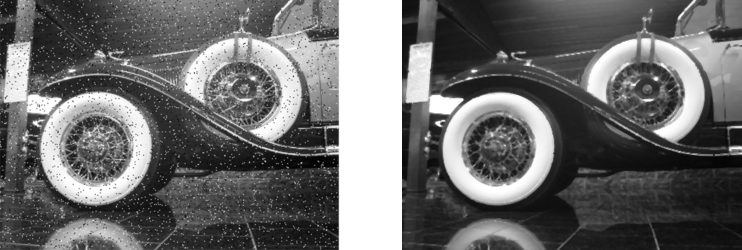
\includegraphics[width=10cm]{filtre-median.png}
\caption{Application du filtre median sur une image bruitée}
\end{figure}

\chapter{Analyse de l'image et extraction des caractères}

\section{Rotation de l'image}

\subsection{Détection de l'angle de rotation}

\subsection{Rotation de l'image}

\section{Segmentation}

\subsection{RLSA}

RLSA (Run Length Smoothing Algorithm) est la méthode que nous avons choisis pour la segmentation des caractères, des lignes et des paragraphes. Elle nous permet en effet de noircir les zones à détecter. Une fois noircies, celle-ci sont ainsi parfaitement isolées du reste de l'image. Par l'exploitation des coordonnées de ces "zones noires" nous pouvons déterminer avec une bonne précision quel est la zone de l'image dans laquelle se trouve un caractère à analyser, une ligne à assembler ou un paragraphe à enregistrer. Nous obtenons ainsi par analyse de l'image noircie la liste des éléments à traiter dans les différentes fonctions que nous écrirons pour la seconde soutenance.

RLSA, fonctionne selon un principe très simple. Il se base sur le postula que l'image qui lui est donnée en entrée est "parfaite". Nous procédons donc avant de l'appeler à tout le pré-traitement de l'image: passage en niveau de gris, application d'un filtre pour faire le flou à l'aide d'une matrice de convolution et une binarisation de l'image avec Otsu. Ainsi, nous obtenons une image où seul les caractères et éventuelles images contiennes des pixels noirs.

Ensuite, il faut analyser l'image deux fois. Nous avons décider de commencer par les rangées puis d'effectuer le traitement en colonne. Ce traitement consiste à faire passer en noir les pixels blancs qui font parti d'un ensemble de pixels noirs. Pour ce faire, nous passons à la fonction un paramètre qui déterminera sous quelle intervalle maximum le nombre de pixels blancs d'affilé doit se trouver pour que ceux-ci passent en noir.

Par exemple, avec un paramètre réglé à 4, la séquence $S$ est transformée en la séquence $C$ :

\begin{align*}
S &= 00010000010100001000000011000\\
C &= 11110000011111111000000011111
\end{align*}

Nous effectuons donc une passe sur chaque rangée, stockons le résultat dans une nouvelle image. Nous passons dans chaque colonne. Ensuite, en considérant le blanc (représenter ici par 1) comme vrai, nous appliquons un ET pour la passe verticale et la passe horizontale. L'image finale est ainsi obtenue et nous pouvons la retourner pour continuer le processus de traitement.

\begin{figure}[htbp]
\centering
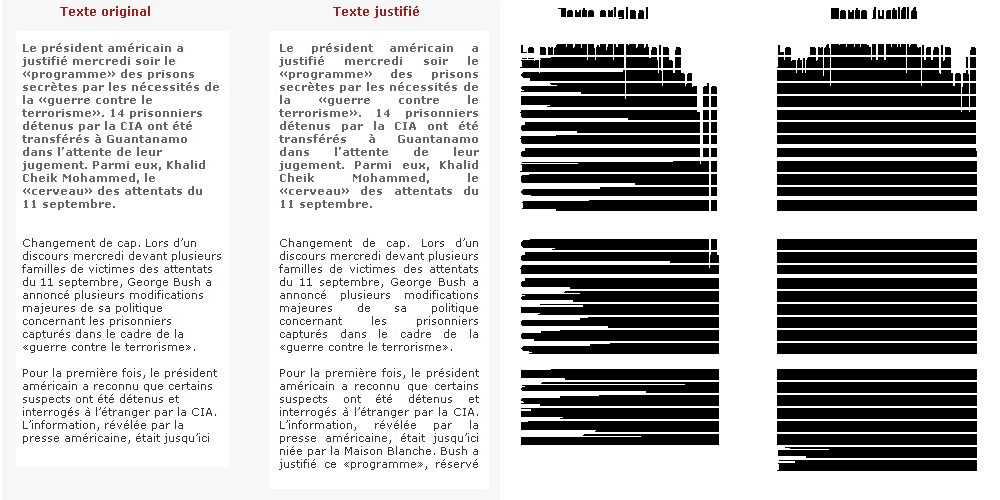
\includegraphics[width=10cm]{rlsa.png}
\caption{Détection des lignes}
\end{figure}

Les avantages de RLSA sont nombreux. En premier lieux, il nous permet de reconnaître les différents éléments de l'image en changeant simplement les paramètres d'appel. Ensuite, grâce à ses deux passes, il fonctionne sur des images droites comme des images penchées. Nous pourrons donc très facilement détecter l'inclinaison à partir de la détection des lignes. Enfin il s'execute dans des temps raisonnables pour des images moyennes ce qui rend son utilisation agréable.

\begin{figure}[htbp]
\centering
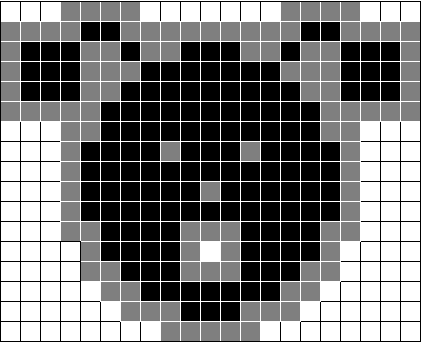
\includegraphics[width=10cm]{dilatation.png}
\caption{Principe de dilatation en morphologie mathématique}
\end{figure}

Cependant, lors de notre avancée dans le projet, nous ne parvenions toujours pas à améliorer l'algorithme afin qu'il détecte de façon convenable les éléments de la page. Ce problème persistant, nous avions décidé d'approfondir nos recherches sur les algorithmes de la famille de RLSA. C'est ainsi que nous avons découvert la morphologie mathématique\footnote{\url{https://fr.wikipedia.org/wiki/Morphologie_math\%C3\%A9matique}} et toute sa complexité. N'obtenant pas beaucoup plus de résultats, nous avons décidé de trouver un autre algorithme.

\subsection{L'algorithme ``maison''}

Pour réaliser la détection des éléments de l'image, nous avons décidé d’implémenter un algorithme au fonctionnement très intuitif : la segmentation successive des paragraphes, lignes et des caractères. Pour ce faire, nous avons utiliser les trois structures de données suivantes.

\bigskip
\lstinputlisting[language=C]{type_segmentation.c}

La première étape est de crée l'histogramme de l'image, il faut effectuer la somme des composantes des pixels de chaque lignes de l'image et les stocker dans un tableau à une dimension. On parcours ainsi ce nouveau tableau, on avance verticalement tant que les colonnes contiennent seulement des pixels blancs. Cela nous à permis de trouver les cotés gauche et droit des différents paragraphes et de mettre à jour les informations contenu dans le struct Bloc. On ajoute l'intégralité des blocs trouvés dans une liste de Bloc.

On parcours ensuite cette liste, on crée l'histogramme de chaque bloc, puis on parcours horizontalement l'image de gauche a droite en ajoutant à la liste incluse dans la structure bloc les lignes trouvées. On parcours à nouveau chaque listes de lignes en créant l'histogramme associé, puis on avance verticalement dans l'image découpant ainsi les caractères afin de les stocker dans les listes associées à la struc Line.

Le gros avantage de cette méthode est que l'on possède dans les structures l'ordre d'envoi les caractères au réseau de neurones pour reconnaître les caractères. En effet, en parcourant la liste de blocs et chaque listes associées aux structures sous jacentes, on obtient les caractères dans l'ordre conventionnelle de lecture. Malheureusement, nous avons rencontré des difficulté pour l'implémenter. Nous avons finalement décidé d'abandonner cette méthode pour utiliser l'algorithme de segmentation XY-Cut.

\subsection{XY-Cut}

L'algorithme de segmentation XY-Cut est un algorithme récursif de découpage de caractère. Il permet à la fois de reconnaître tout type de blocs mais aussi, une fois amélioré, de reconnaître l'ordre de lecture des paragraphes\footnote{\url{http://pdf.aminer.org/000/295/221/optimized_xy_cut_for_determining_a_page_reading_order.pdf}}. Nous avons choisi d'utiliser cette méthode pour notre OCR.

Son principe est de s'appeler alternativement sur un mode horizontal et vertical. A chaque appel, XY-Cut découpera l'image autour des cadres contenants des éléments de l'image.

\begin{figure}[htbp]
\centering

\includegraphics[width=10cm]{1.png}
\caption{Illustration du fonctionnement de XY-Cut (1/3)}
\end{figure}

La longueur ``a'' correspond à la constante a partir de laquelle nous considérons que le cadre ne contiens plus qu'un caractère. Si le cadre envoyé en paramètre à XY-Cut est plus petit sur sa composante verticale et sur sa composante verticale, alors nous considérons que nous sommes en présence d'un caractère.

Le resserage de XY-Cut autour de l'élément à détourer se déroule de façon simple. Considérons que nous sommes sur un appel vertical. La fonction XY-Cut génère en premier lieu un vecteur contenant la somme des valeurs de toutes les colonnes de l'image. La fonction s'appelle ensuite en mode horizontal sur chaque cadre contenant au moins un pixel noir. Les zones blanches sont ainsi entièrement éliminées du processus.

\begin{figure}[htbp]
\centering

\includegraphics[width=10cm]{2.png}
\caption{llustration du fonctionnement de XY-Cut (2/3)}
\end{figure}

Le processus est répété sur chacune des zones permet ainsi de se rapprocher un peu plus à chaque appel de XY-Cut. Une fois que le cadre est suffisamment réduit, nous envoyons celui-ci au réseau de neurones. Nous avions initialement prévus de stocker le résultat des appels dans un arbre général afin de pouvoir traiter les caractères dans l'ordre mais l'utilisation de l'arbre s'est révélée inutile. En effet, dans notre cas, l'utilisation d'une liste suffit à conserver l'ordre des caractères.

\begin{figure}[htbp]
\centering

\includegraphics[width=10cm]{3.png}
\caption{llustration du fonctionnement de XY-Cut (3/3)}
\end{figure}

\chapter{Reconnaissance des caractères}

\section{Réseau de neurones}

%TODO : modif structure, enregistrement dans un fichier, apprentissage, resultat

\subsection{Principe de base}

Un réseau de neurones se compose, comme sont nom l'indique, de plusieurs neurones connectés entre eux. Chaque neurone à un ou plusieurs liens entrants et sortants. Ces liens, aussi appelés liaisons, sont affectés par des poids qui permettent de définir l'importance d'une liaison entre deux neurones par rapport à une autre. De plus, on rajoute à cela une fonction d'activation qui définie en fonction des variables d'entrées si un neurone est actif ou non. Le résultat de la fonction d'activation est renvoyé en sortie du neurone. On choisi généralement une fonction d'activation qui renvoie des valeurs entre $[0; 1]$ ou $[-1; 1]$.

\begin{figure}[htbp]
\centering
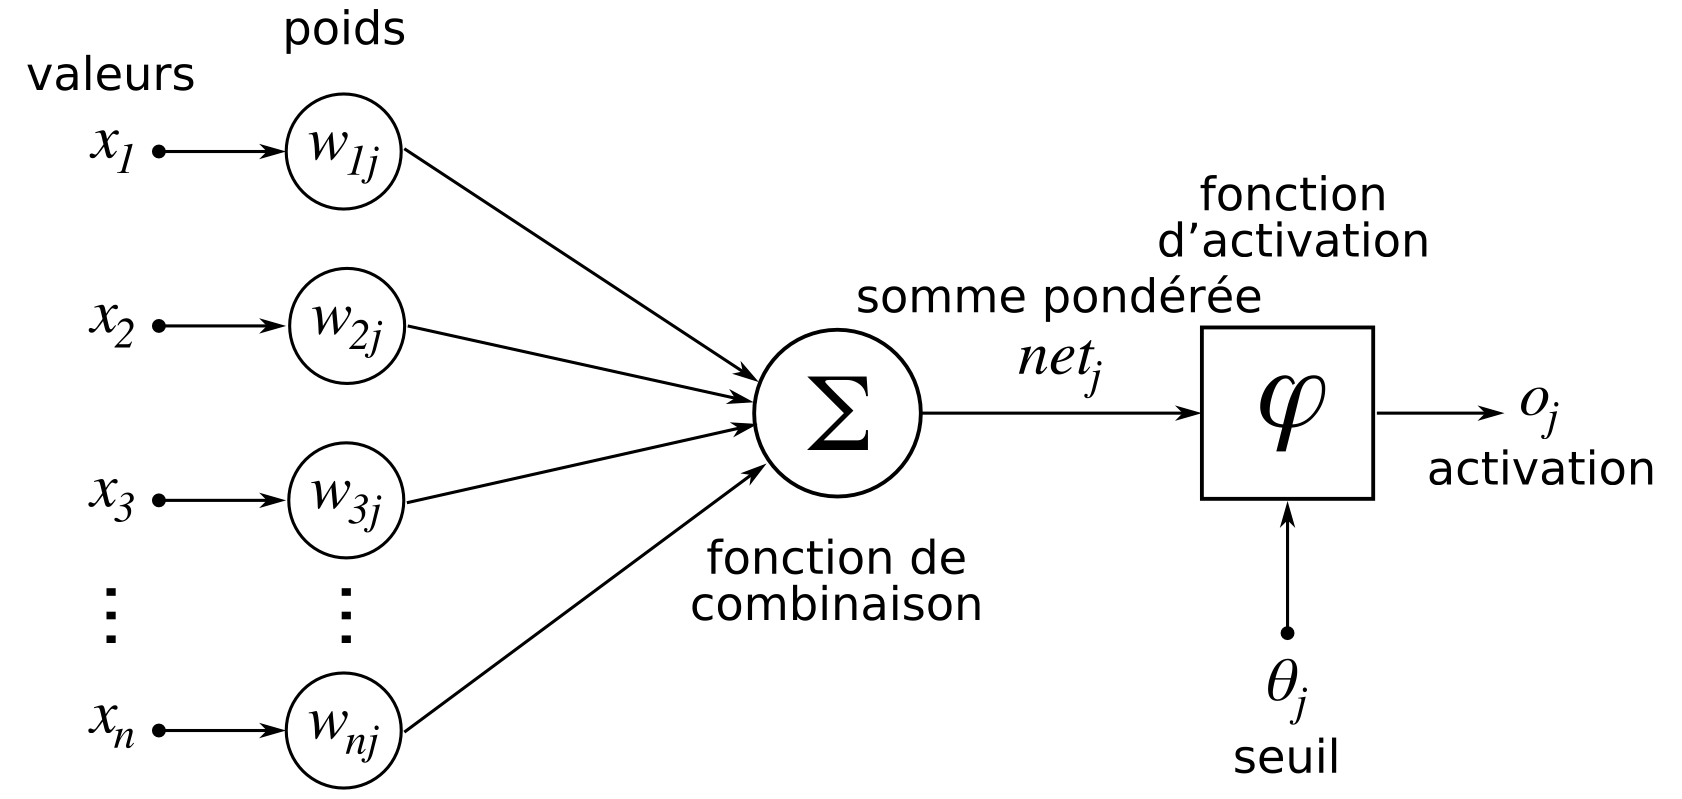
\includegraphics[width=10cm]{perceptron.png}
\caption{Schéma d'un neurone}
\end{figure}

\subsection{Structure du réseau}

Un réseau de neurones est en général composé d'une succession de couches dont chacune prends ses entrées sur les sorties de la couche précédentes. Une couche est composée de $N_{i}$ neurones, prenant leurs entrées sur les $N_{i-1}$ neurones de la couche précédente. Cependant, on peut retrouver d'autre type de formation comme les réseaux Hopfield.Dans la suite de cette partie, nous ne nous intéresserons qu'au réseau de type MLP, Multi-Layer Perceptron, car c'est ceux-ci que nous utiliserons pour le projet.

\begin{figure}[htbp]
\centering
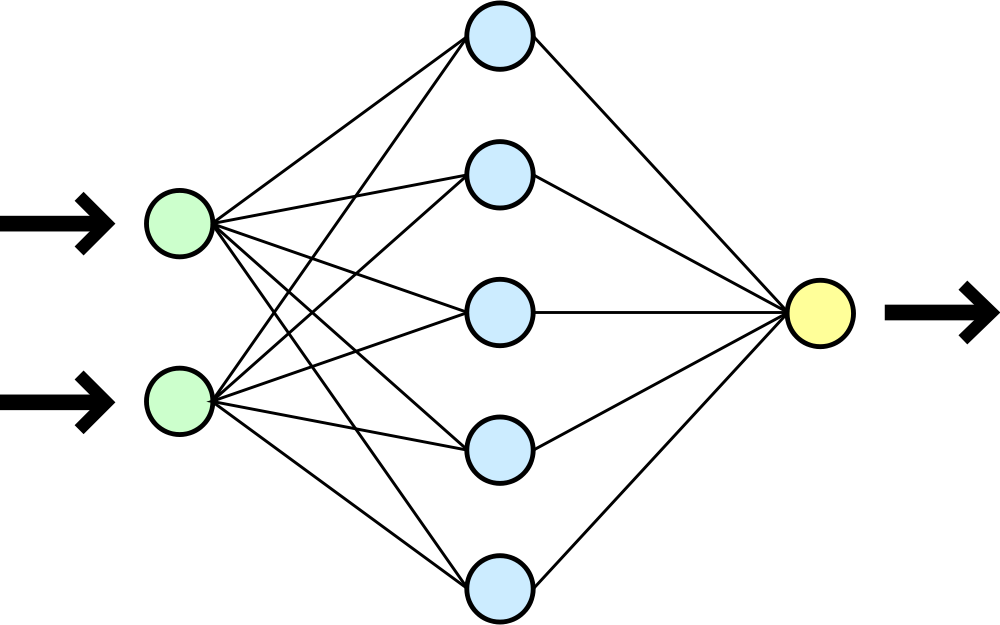
\includegraphics[width=10cm]{mlp.png}
\caption{Schéma d'un réseau de type MLP}
\label{MLP}
\end{figure}

Sur le schéma de la figure~\ref{MLP}, on peut constater que le réseau de neurones est constitué de trois couches. La première couche, en vert, est composé de deux neurones d'entrée. C'est à ceux-ci que l'on passera nos valeurs d'entrées brutes. En bleu, il s'agit de la couche caché. Et enfin en jaune on trouve la couche de sortie qui nous retourne donc le résultat du réseau de neurones.

\subsection{L'apprentissage}

Il existe plusieurs modes d'apprentissage pour les neurones. Tout d'abord il y a l'apprentissage supervisé. Dans ce type d'apprentissage, le réseau de neurones s'adapte en comparant le résultat qu'il a calculé et le résultat attendue. Le réseau de neurones va donc se modifier petit à petit jusqu'à qu'il atteigne la bonne configuration.

Il existe une autre méthode qui s'appelle le renforcement. Dans celle-ci, le réseau de neurone doit apprendre à faire un rapport entre les entrée et les sorties grâce à une estimation de son erreur. C'est-à-dire que le réseau va optimiser un index de performance qu'on lui donne et qui va lui permettre de savoir si la réponse est bonne ou non, mais sans connaître la  bonne réponse.

Dans notre configuration, nous utiliserons l'apprentissage supervisé. Pour cela nous avons besoin de la technique de rétropropagation, aussi appelé rétropropagation du gradient. Cette méthode permet de calculer le gradient de l'erreur de chaque neurone, de la dernière couche à la première.

L'algorithme est simple à comprendre. On commence par calculer l'erreur de la ou les sorties $i$. Pour cela on utilise la formule :

\[ erreur(i) = S_{desiree} - S_{obtenue} \]

Ensuite on parcours chaque couche du réseau, en partant de la couche de sortie, en propageant l'erreur de la couche $k$ à la couche $(k-1)$ par les liens synaptiques. La figure~\ref{retropropagation} illustre brièvement le fonctionnement de l'algorithme.

\begin{figure}[htbp]
\centering
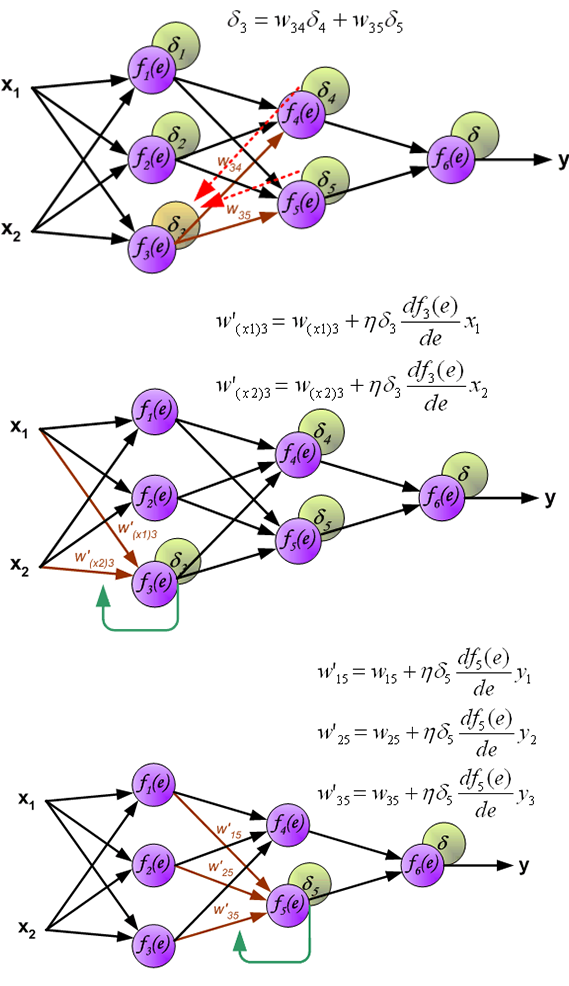
\includegraphics[width=10cm]{retropropagation.png}
\caption{Calcul de rétropropagation}
\label{retropropagation}
\end{figure}

\subsection{Implémentation}

\subsubsection{Structure de donnée}

Pour la représentation en mémoire de notre réseau de neurone, nous utilisons trois types différents. Le premier s'appelle $t\_neuron$. C'est celui-ci qui représente un neurone en mémoire. Chaque neurone possède une sortie, un bias (sauf les neurones de la couche d'entrée) et une liste de liens synaptiques.

Le type $t\_connection$ représente un lien. Il possède un poids et deux champs de type $t\_neuron$ représentant les deux neurones reliés par le lien.

Enfin, le type $t\_network$ représente en mémoire notre réseau de neurones au complet. Il possède un pointeur vers l'ensemble des neurones, organisé en différentes couches.

\bigskip
\lstinputlisting[language=C]{type_structure.c}

\subsubsection{Fonction d'activation}

Pour la fonction d'activation, nous avons choisi d'utiliser la fonction mathématique sigmoïde. En effet, celle-ci est souvent utilisé par les réseaux de neurone du fait de ses caractéristiques : sa forme en S et son équation différentiel simple à calculer (utile pour la rétropropagation). Elle est défini par :

\[ f\left( x\right) = \dfrac{1}{1+e^{-x}} \]

Son équation différentiel est :

\[ \dfrac{dy}{dx} = y\left(1-y\right) ; y \in [0; 1] \]

\begin{figure}[htbp]
\centering
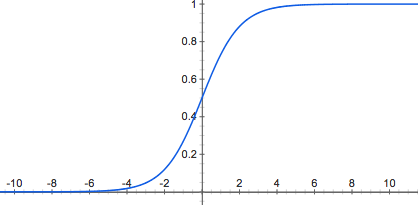
\includegraphics[width=10cm]{sigmoide.png}
\caption{Courbe de la sigmoïde}
\end{figure}

\subsubsection{Fonction de combinaison}

Vue que nous utilisons un réseau de type MLP, notre fonction de combinaison renvoie le produit scalaire entre le vecteur de valeurs d'entrée d'un neurone et le vecteur des poids des liens synaptiques. C'est-à-dire :

\[ a_{j} = \varphi \left( \left( \sum_{i} w_{ij} x_{i} \right) + b_{i} \right) \]

\begin{description}
\item[$a_{i}$] : valeur de sortie du neurone $j$.
\item[$\varphi$] : fonction d'activation.
\item[$w_{ij}$] : poids du liens synaptiques entre le neurone $i$ et $j$.
\item[$x_{i}$] : valeur de sortie du neurone $i$ de la couche précédente.
\item[$b_{i}$] : bias du neurone $j$.
\end{description}

\subsection{Un exemple d'utilisation : XOR}

Pour cette soutenance, nous avons utilisé notre implémentation du réseau de neurones pour lui faire apprendre la fonction XOR. Le réseau de neurones est composé de deux neurones d'entrées, deux neurones sur la couche caché et un neurone de sortie.

\begin{figure}[htbp]
\centering
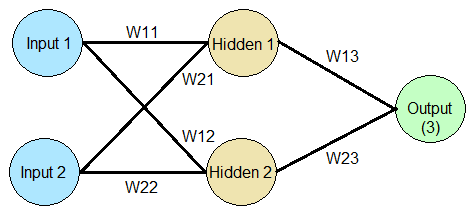
\includegraphics[width=6cm]{xor_neuron.jpg}
\caption{Réseau de neurones utilisé pour le XOR}
\end{figure}

Comme on peut le voir sur la figure~\ref{xor}, le réseau de neurones apprends par rétropropagation à répondre correctement. Au bout d'un certain nombre de cycle d'apprentissage (appelé aussi epoch), le réseau de neurone est capable de reproduire la fonction XOR sans se tromper.

\begin{figure}[htbp]
\centering
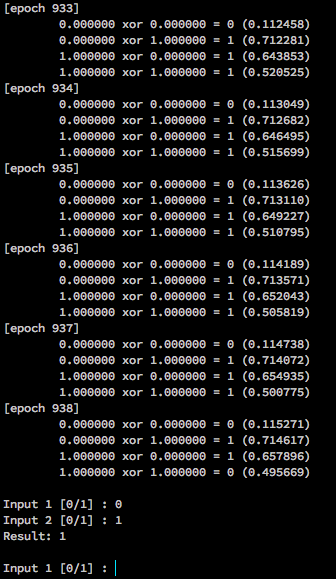
\includegraphics[width=6cm]{xor.png}
\caption{Apprentissage de la fonction XOR par notre réseau de neurones}
\label{xor}
\end{figure}

\chapter{Interface graphique}

La réussite d’un programme informatique se base sur deux choses : le résultat qu’il produit et son accessibilité. Il serait dommage de limiter l’utilisation d’un outil informatique à une poignée de personnes uniquement à cause d’un aspect spartiate - le shell par exemple - qui décourage beaucoup de néophytes. C‘est pourquoi l’interface graphique, GUI (pour Graphical User Interface), est un point majeur de tout projet ayant pour ambition de toucher un public large et varié.

Nous avons donc décidé de concevoir l’interface graphique d’OhÇaSert à l’aide de la bibliothèque GTK-3.0. Nous avons utilisé sa version dans le langage C bien évidement. Le logiciel Glade a aussi fait partie des outils utilisés pour développer cette interface, cela pour plusieurs raisons. Glade nous permet de créer une interface suffisamment esthétique d’un point de vue visuel direct. S’il est certes possible d’obtenir le même résultat sans, cela est plus difficile et surtout plus long. La seconde raison complète la première : nous pouvons opérer des changements à la volée sur notre interface sans devoir re-compiler, ce qui est un gain de temps non négligeable.

\section{Les différentes fenêtres}

Si notre interface ne prétend pas être d’un esthétisme professionnel (le dessin n’a jamais été notre fort), elle se suffit parfaitement à l’utilisation d’un OCR : sobriété et efficacité sont notre credo. Ainsi notre interface est composée principalement d’une zone où est affichée l’image choisie et d’une zone de texte où afficher le résultat de notre OCR.

\begin{figure}[htbp]
\centering
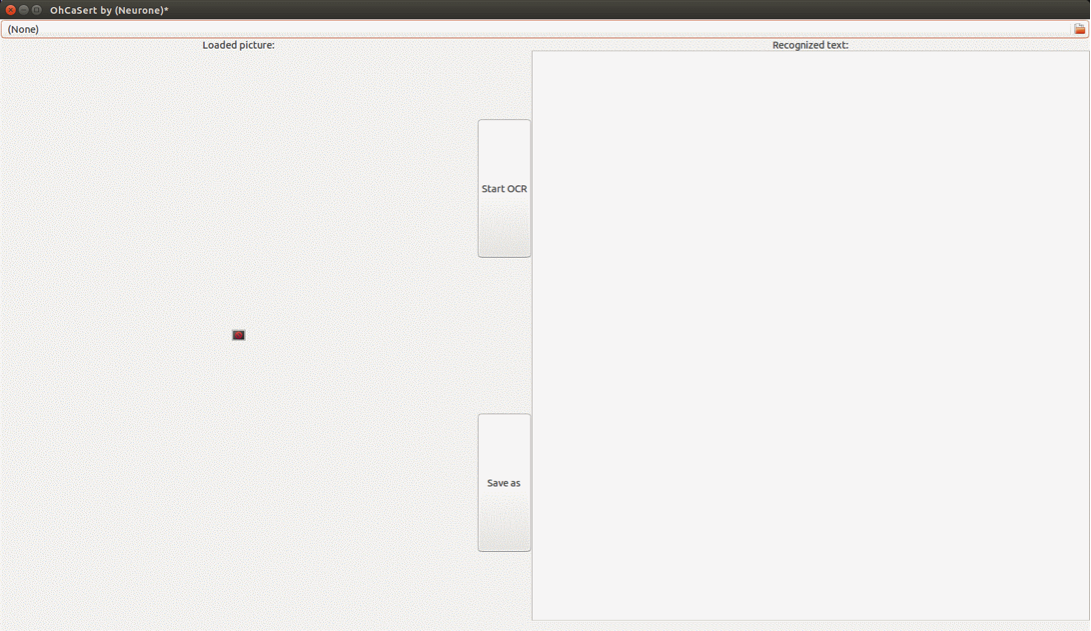
\includegraphics[width=10cm]{gui.png}
\caption{Fenêtre principale}
\end{figure}

La première longue barre horizontale est la barre menu, dans l’onglet FILE se trouve les fonctions ``Save as'' et ``Quit''. Dans l’onglet EDIT, la fonction ``Delete'' permet de supprimer l’intégralité du texte se trouvant dans la zone de texte. Et enfin dans l’onglet HELP se trouve la fonction ``About''. Celle-ci ouvre une nouvelle fenêtre sur laquelle on peut retrouver la version du programme actuellement utilisé et un lien vers notre site web.

\begin{figure}[htbp]
\centering
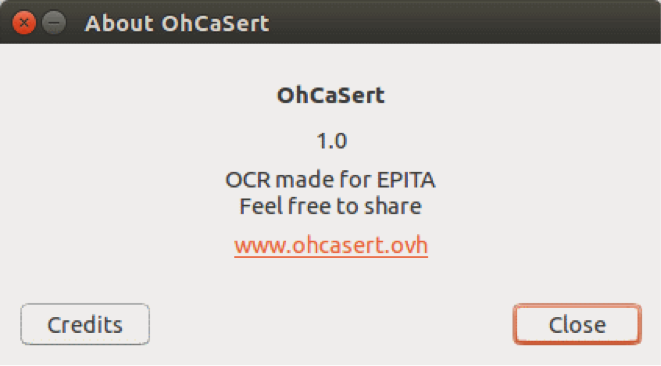
\includegraphics[width=10cm]{gui-about.png}
\caption{Fenêtre ``About''}
\end{figure}

Sur cette dernière fenêtre, vous trouverez également un bouton ``Credits''. Celui-ci permet de lister les logins des développeurs de ce projet.

\begin{figure}[htbp]
\centering
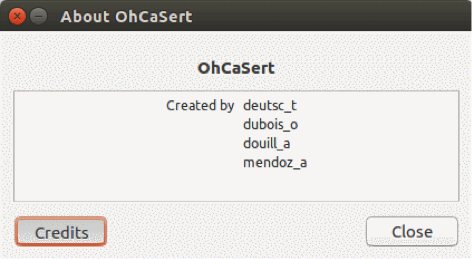
\includegraphics[width=10cm]{gui-credits.png}
\caption{Fenêtre ``Credits''}
\end{figure}

\section{Le fonctionnement}

L'utilisation de l'application est très simple et intuitive. L'utilisateur doit tout d'abord cliquer sur la grande barre horizontale. Celle-ci lui permet de sélectionner une image parmi ses documents.

\begin{figure}[htbp]
\centering
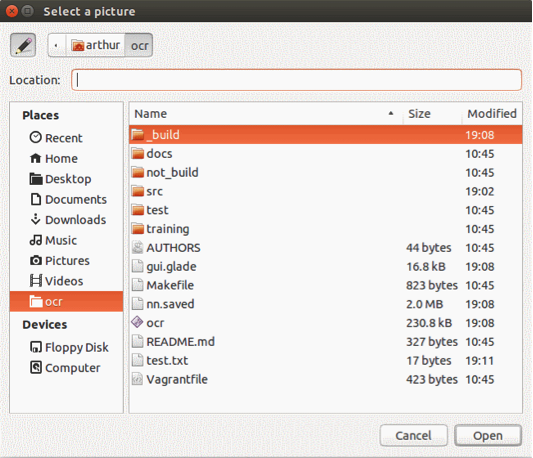
\includegraphics[width=10cm]{gui-open-file.png}
\caption{Fenêtre permettant de charger une image}
\end{figure}

Ce gestionnaire de fichier récupère le chemin d'accès vers l’image et l’affiche dans la zone prévue à cet effet à l'aide du widget GtkImage. L'image chargé est redimensionné à la taille du dit widget via les fonctions de GtkPixbuf.

Le bouton ``Start OCR'' exécute l'ensemble du processus d'analyse de l'image, de la segmentation et de la reconnaissance de caractère de notre OCR. Le résultat de l'analyse de l'image et de son traitement est alors affiché à la place de l'image original et le texte reconnu est inséré dans la zone prévu à cet effet.

\begin{figure}[htbp]
\centering
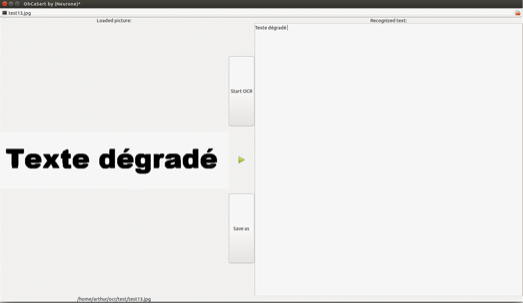
\includegraphics[width=10cm]{gui-result.png}
\caption{Résultat final affiché dans l'interface}
\end{figure}

S’il y a des erreurs dans le texte généré, venant soit du texte original ou bien d’une mauvaise détection, le mot incriminé sera souligné en rouge. Un simple clic-droit dessus proposera diverses suggestions de correction. Le correcteur orthographique est par défaut en français, mais un simple clic-droit dans la zone de texte permet de changer de langue. Pour utiliser ce correcteur orthographique, il est nécessaire d'avoir installer sur sa machine les bibliothèques GtkSpell et Aspell-fr.

Enfin, l'utilisateur peut choisir de sauvegarder le texte grâce au bouton  ``Save as''. Celui-ci lui permet de sélectionner une destination et un nom de fichier.

\begin{figure}[htbp]
\centering
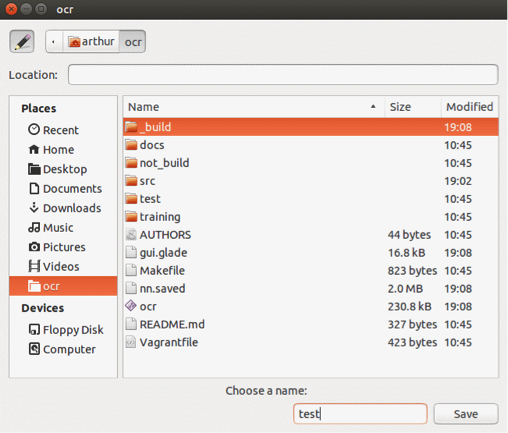
\includegraphics[width=10cm]{gui-save.png}
\caption{Fenêtre permettant de sauvegarder le résultat}
\end{figure}

\chapter{Site web}

\section{Conception du design}

Le site a été conçu avec Bootstrap, un framework HTML/CSS/Javascript qui permet de concevoir très rapidement des sites internet avec de nombreuses fonctionnalités. Mais le grand intérêt de ce type de framework c’est qu’ils sont pensés pour être “responsive design” et qu’ils s’affichent à l’identique sur l’ensemble des navigateurs internet.

Le design s'inspire d'un effet de mode : ``scrolling website''. Cela consiste à faire tenir tout les informations sur une seule page, de manière esthétique, que l'utilisateur fera défiler (en anglais scroll) de haut en bas. De plus nous avons décidé d'adopter une palette de couleur sombre pour rappeler la couleur des textes et de l'encre : noir.

L'image d'accueil que nous avons choisit pour illustrer notre projet est un dessin d'un livre dont les lignes, les mots, les morceaux de phrases forment un dédale surprenant. La première idée qui nous vient en voyant cette image est évidemment le découpage des paragraphes, des lignes et des caractères: un des aspects majeurs de tout OCR qui se respecte.

\begin{figure}[htbp]
\centering
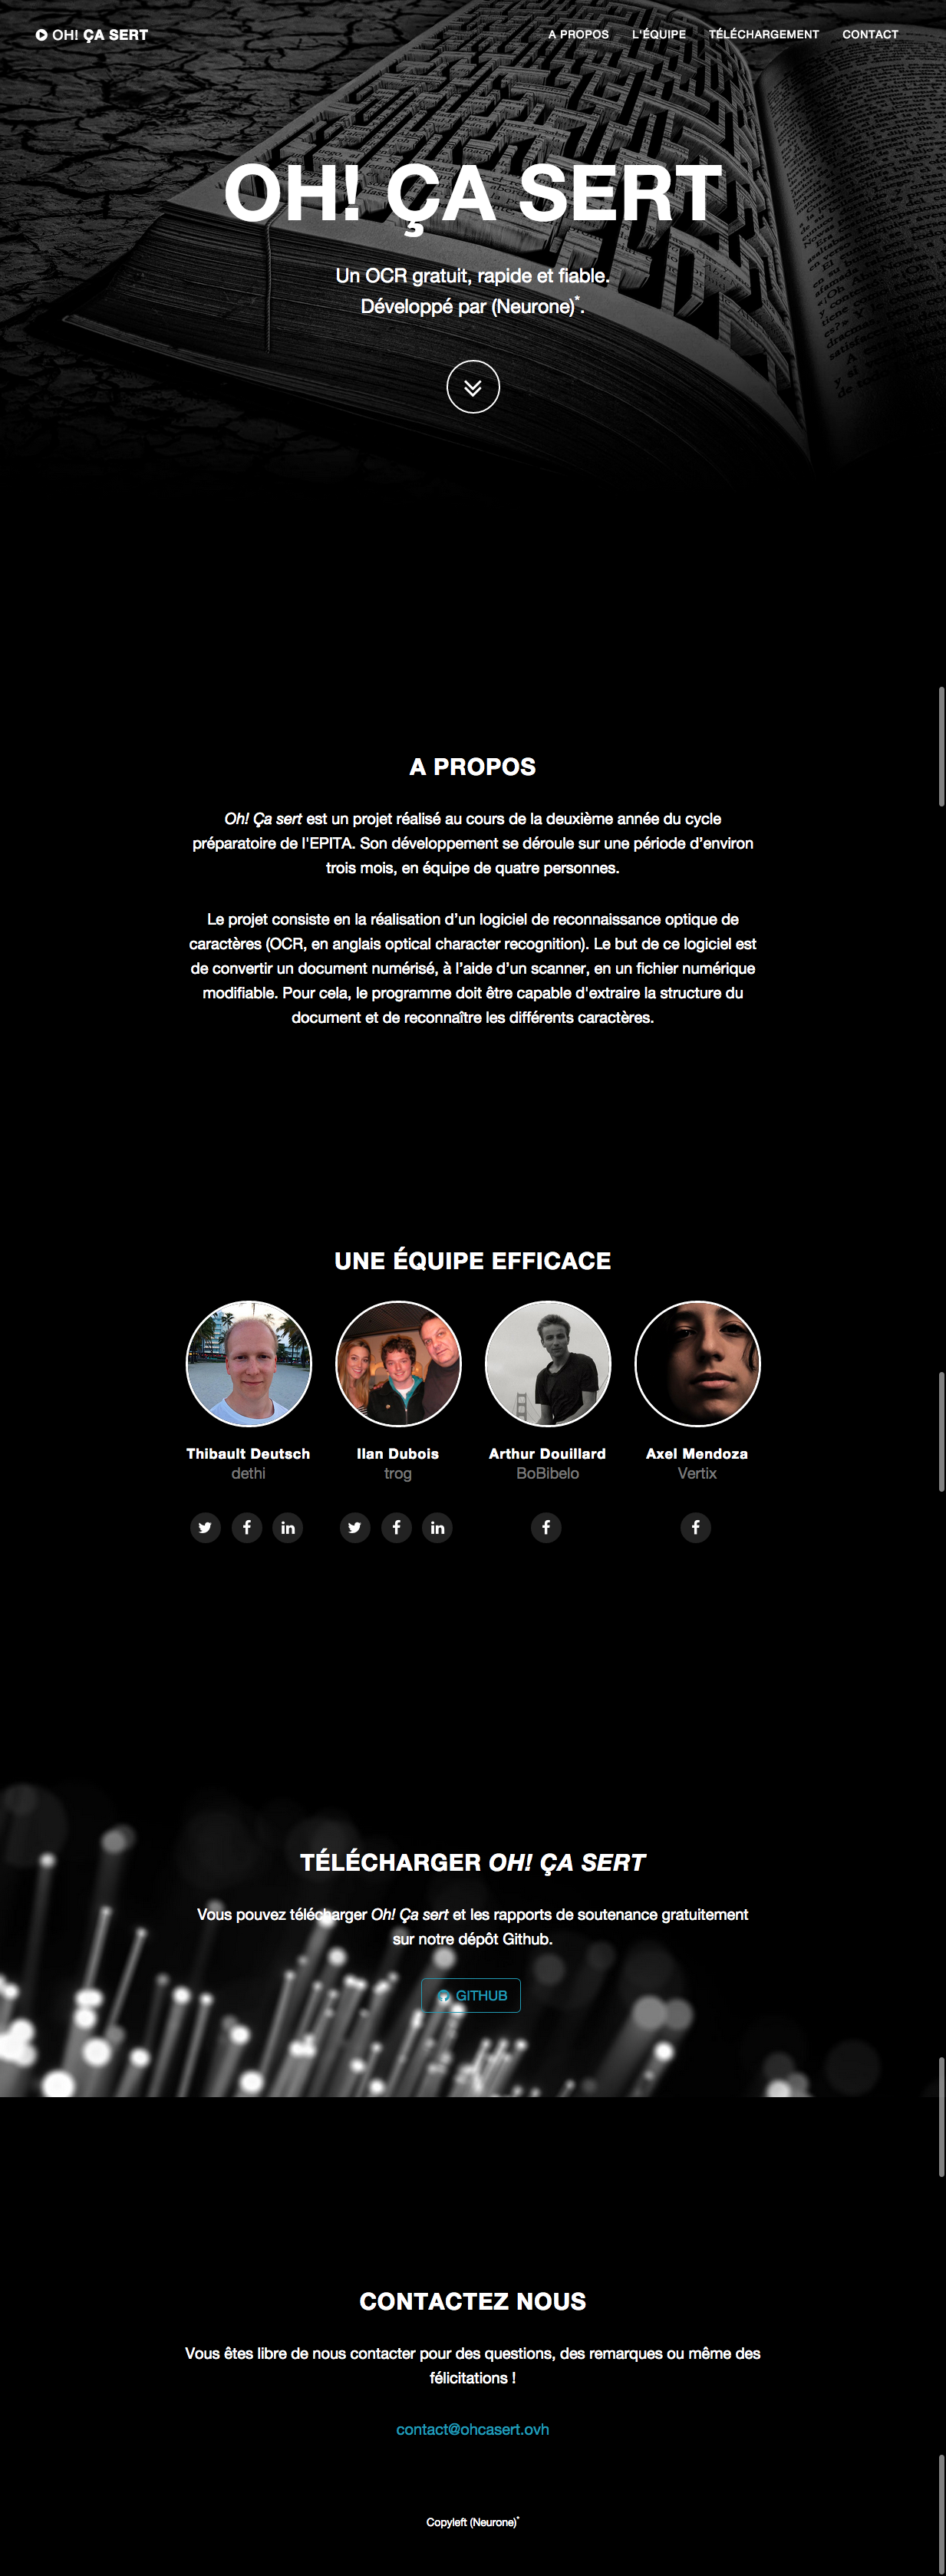
\includegraphics[height=20cm]{www.png}
\caption{Notre site web}
\end{figure}

\section{Contenu et accès au site web}

Le site web consiste en une seule page que l'on fait défiler du haut vers le bas. On y trouve les informations suivantes :

\begin{itemize}
\item La page d’accueil, permettant d'accéder à l'aide de liens aux différentes parties du site. On peut aussi y trouver le nom du groupe instigateur du projet et son slogan.
\item Une partie ``à propos'' qui présente rapidement les enjeux du projet.
\item Une partie ``équipe``, listant les membres du groupe ainsi que des liens vers les réseaux sociaux.
\item Une partie essentielle : celle dédiée au téléchargement de notre OCR, que l'on peut effectuer très aisément à l'aide du lien fourni.
\item Une partie ``contact'' si vous désirez joindre un de nos membres, pour des questions, des remarques ou bien même des félicitations !
\end{itemize}

Notre site internet est accessible à l'adresse \url{http://www.ohcasert.ovh}.

\chapter{Synthèses personnelles}

\section{Thibault}

%TODO

\section{Ilan}

Au cours de la réalisation de ce projet, j'ai eu l’opportunité d'apprendre de très nombreuses choses sur le C et sur le traitement d'image. En ce qui concerne le C, les notions que j'ai découvertes sont très enrichissantes. J'ai appris à utiliser GDB qui s'est souvent révélé extrêmement utile. Notamment, lors de la réalisation de la segmentation des caractères. J'ai aussi eu l'occasion de mieux comprendre comment fonctionnait la gestion de la mémoire sur un système UNIX. Ces notions seront utiles pour la suite de on cursus, notamment en ING1.

En terme de traitement d'image, j'ai eu l'occasion d'apprendre des algorithmes come XY-Cut. En outre, j'ai eu 'occasion de découvrir des notions plus avancées tel que la morphologie mathématique.

De plus, ce projet m'a appris beaucoup de choses en terme de gestion de projet à plusieurs. Je pense maintenant pouvoir définir plus facilement les priorités lors de la réalisation d'un projet. Ma façon de gérer le temps a elle aussi été impactée par ce projet, elle et désormais plus optimale.

\section{Arthur}

Le projet OhÇaSert, destiné à concevoir un OCR, m’a beaucoup apporté sur des plans aussi nombreux que variés.

Premièrement, étant donné que c’est ma première année à l’EPITA, je n’avais jamais pu participer à un projet d’informatique en groupe de cet ampleur avant celui-ci. Ce fut donc pour moi une expérience radicalement nouvelle et pour ainsi dire passionnante.

En Septembre, à la rentrée je tâtonnais sur Linux, je bafouillais deux trois lignes de codes en C, mais voilà que l’OCR a fait de moi, à défaut d’un homme meilleur, un meilleur développeur : J’en suis venu à préférer, à ma propre surprise, Linux et plus particulièrement Ubuntu face à Windows. Le shell c’est le bien, voilà ce que j’ai retenu. L’existence même de malloc/calloc et autres joyeusetés me semblait confuse, maintenant je peux malloc() à tour de bras (mais pas toujours correctement encore, mais ça viendra !). N’ayant pratiqué que du python auparavant, cette gestion de la mémoire m’a en effet surpris au départ, mais j’en suis venu à l’apprécier, et je pense sérieusement continuer à pratiquer le C lors de mon voyage à l’étranger au S4 pour être prêt pour l'ING1.

Outre l’aspect purement pratique que cette expérience, ce projet m’a appris à gérer mon temps afin d'éviter le rush, même si ce celui se révéla obligatoire et malgré quelques appréhensions excitant. En plus d’une gestion améliorée du temps j’ai aussi appris le travail en équipe, via Git, via des conversations Mumble interminables, traquant le bug dans ces moindres recoins. J’ai aussi appris qu’un groupe était autant source d’aide pour moi, que moi pour eux : ce fut un échange réciproquement et équitable d’information entre mes camarades qui nous a permit d’éliminer des tracasseries dans nos codes, et nous valant des nuits blanches en groupes.

\section{Axel}

Après la première soutenance, je me suis consacré à continuer l'implémentation du pré-traitement et une partie de la segmentation de l'image.
Je me suis tout d'abord occupé d’implémenter un filtre médian, qui m'as parut plus efficace pour supprimer les grains importants du bruit.
Par la suite, j'ai aidé Ilan à débugger son algorithme de segmentation de l'image en caractère XY-cut. 
J'ai tenté une nouvelle approche du problème de la segmentation en blocs lignes et caractères mais Ilan a réussit à faire fonctionner XY-cut donc la méthode que j'ai utiliser n'as pas aboutit.

Malheureusement, j'ai rencontré de nombreux problèmes lors de la finalisation de notre projet, par conséquent très peu de mon code à été utilisé dans la partie fonctionnelle de notre OCR.
Je ne suis pas déçu ni décourager pour autant suite à cette expérience de groupe car même si la plupart de mes algorithmes n'ont pas aboutit, j'ai appris beaucoup de choses qui me servirons probablement pour l'année prochaine.
Pour finir, je suis très content d'avoir former un groupe avec mes partenaires de projet car nous avons su nous délégué les différentes tâches et nous aider les uns les autres.
Même si la finalisation de notre projet n'as pas été à la hauteur de nos attentes, je ne regrette rien et je suis prés pour de nouveaux projets informatiques après mon voyage en Corée !

\chapter{Conclusion}

%TODO

Nous sommes contents des fonctionnalités que nous avons réalisées pour cette première période de travail. Dans l'ensemble, le cahier des charges a été respecté. Mais il reste encore beaucoup de travail à réaliser, notamment au niveau de l'extraction et de la reconnaissance des caractères.

Nous partons confiants pour la suite du projet. En effet, nous avons déjà réaliser pas mal de recherche pour la suite. Il ne nous reste plus qu'à implémenter et comparer les différents algorithmes que nous avons trouvés ces derniers jours.

\newpage
\pagenumbering{Roman}
\part*{Annexes}

\newpage
\listoffigures
 
\end{document}
